HTBAC % by design 
allows to % represents 
encode binding free energy protocols, such ESMACS and TIES\@. We model a
protocol using a series of simulation steps and assigning the number of
replicas\mtnote{I am not sure I understand this sentence: to what do we
assign one or more replica?}. We express the application logic of HTBAC using
the user-facing API % components 
of EnTK (\S\ref{ssec:entk}). 

EnTK % provides a common 
API and programming model allow HTBAC to express the workflows associated
with different protocols as ensemble-based applications,
% uniformly, and thus 
minimizing development effort and complexity. 
% We describe these components for the ESMACS protocol\@. 
% Typically, a protocol % typically 
% corresponds to a single physical system. 
The concept of % an 
ensemble in the ESMACS \mtnote{and TIES? You mentioned it above. At some
point we will have to transition to ESMACS only but the transition needs to
be justified.} protocol maps directly to a set of pipelines in EnTK, where
each pipeline contains functions that operate on a given replica. EnTK
interprets these replicas as independent pipelines. Each pipeline consists of
multiple stages representing a well-defined execution order; each stage can
contain heterogeneous workloads. Although each stage of a pipeline depends on
its predecessor, the pipelines execute independently of each other. The
patterns within pipelines are identical and describe an ensemble of replica
simulations, as shown in Fig~\ref{figure:HTBAC}.\mtnote{I am afraid we need
to iterate the whole pragraph. We need to separate between the abstracitons
used in the ESMACS protocol (replica, function, simulation) to those of EnTK
(pipeline, stage and task). Once separated, we need to map the former into
the latter.}

\begin{figure}
\centering
  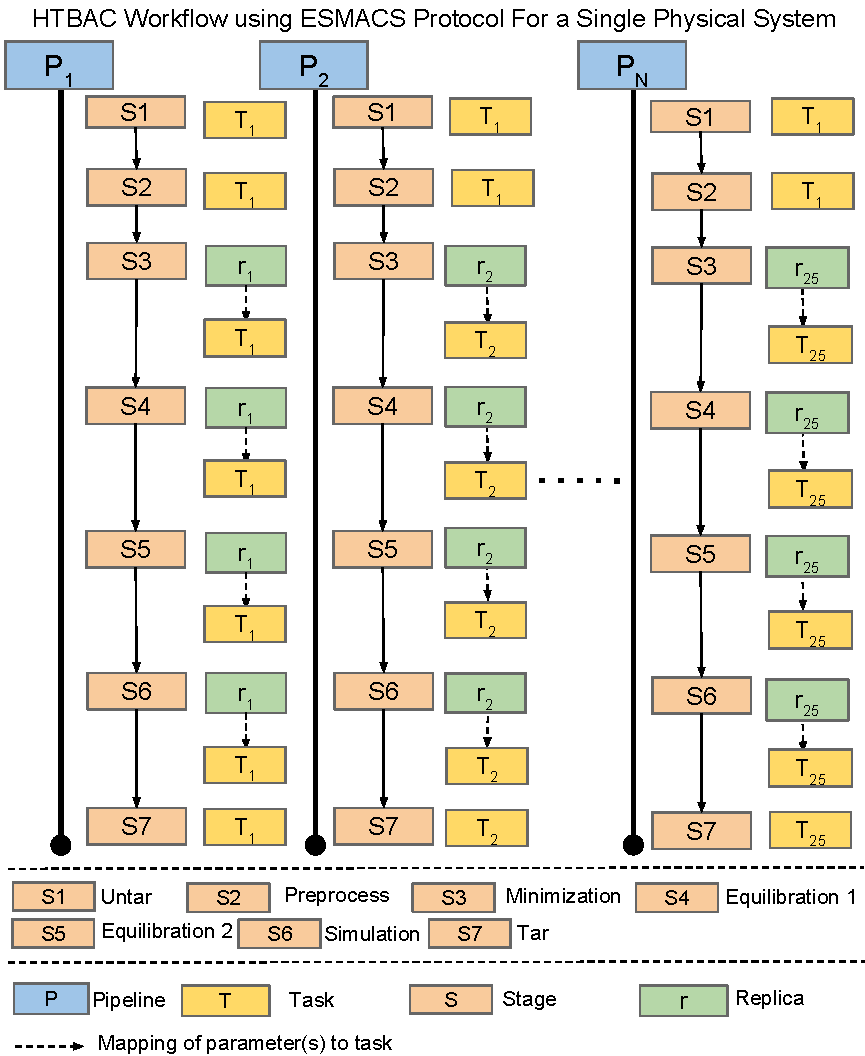
\includegraphics[width=0.5\textwidth]{FIGURES/HTBAC_Workflow_ESMACS.pdf}
  \caption{ESMACS protocol implemented as an HTBAC workflow, encoded using
  the EnTK PST model. Each protocol represents a physical system and is
  captured as a set of independent pipelines. Each pipeline maps to a single
  replica. Stages within a pipeline maintain temporal ordering. Each stage
  contains a single task. Stages S3-S6 contain NAMD
  tasks.}\label{figure:HTBAC}
\end{figure}

The ESMACS protocol consist of pipelines with stages comprised of
heterogeneous tasks. For example, equilibration and production, followed by
post processing steps. The different protocols differ in the details of the
pipelines, stages and synchronization~\cite{Bhati2017}.

% \begin{figure}
% \centering
%   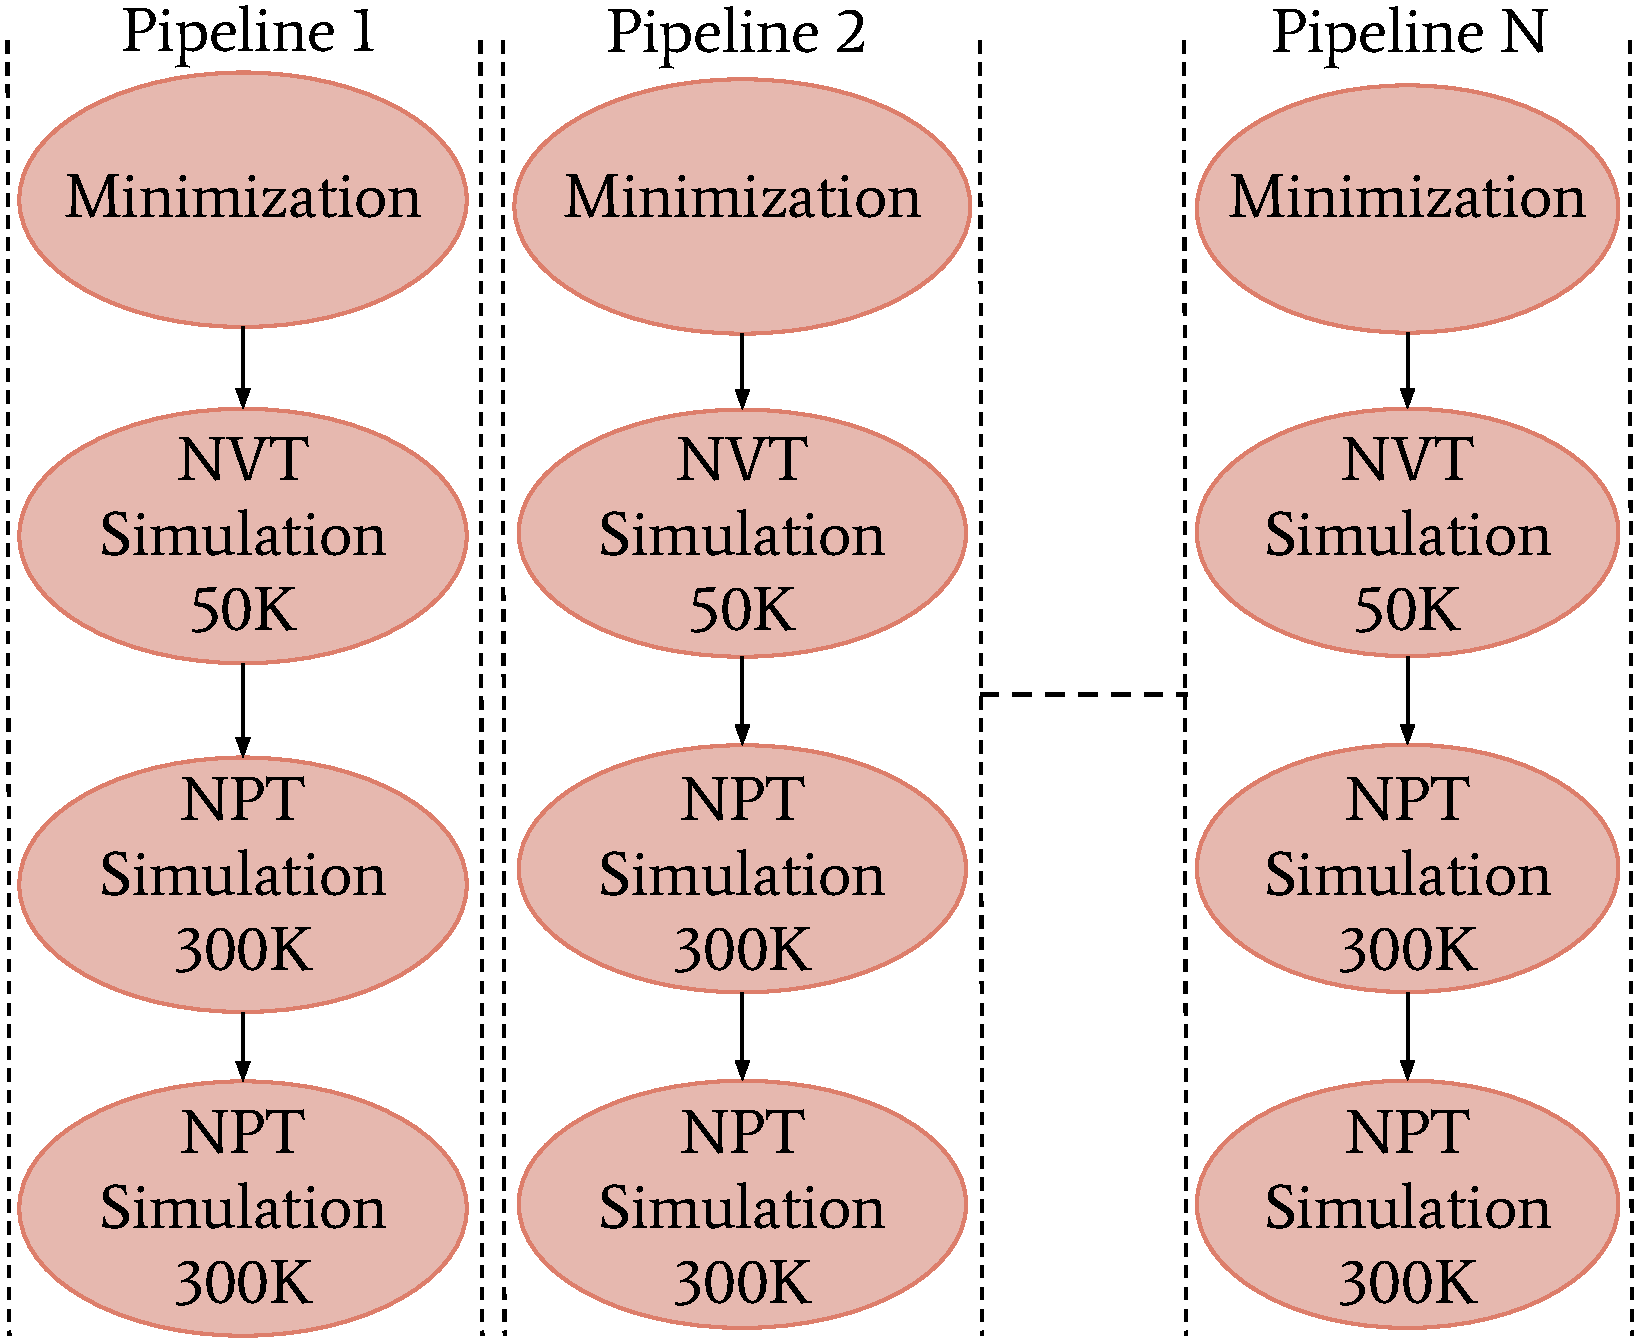
\includegraphics[width=0.5\textwidth]{FIGURES/HT-BAC_NAMD_pipelines_control_flow_only.pdf}
%   \caption{ESMACS protocol indicating how an N replica ensemble is implemented in HTBAC.
%   Each protocol instance is mapped to a single EnTK pipeline.
%   Each pipeline is equivalent and represents a set of simulations which are captured as stages by
%   EnTK.}\label{figure:ESMACS-pipelines}
% \end{figure}

%\begin{itemize}
%	\item 1) Untar configuration files
%	\item 2) Preprep
%	\item 3) Minimize with decreasing restraints
%	\item 4) Equilibration: NVT simulation at 50K, with restraints
%	\item 5) Equilibration: NPT simulation at 300K, with decreasing
%	restraints
%	\item 6) Equlibratin: NPT at 300k, no constraints
%	\item 7) Tarball output files
%\end{itemize}

Each stage is composed of a single unique task which is described by a set of
attributes that define the workload parameters such as the location of input
files, the number of simulations and the MD engine(s) to launch simulations.
The ESMACS protocol defines 7 stages, in which the first and last
stages perform staging of the input/output data. The middle stages indicate
simulation tasks as shown in Fig~\ref{figure:HTBAC}. The task is
appended to a stage and stages are appended to a pipeline to maintain
temporal order. The workflow relies on a resource configuration which
consists of the details required to use a resource where the application will
be executed including runtime, queue, and account details. We capture the
integration of the application (ESMACS protocol) and how it interfaces with
EnTK in Fig~\ref{figure:ht-bac_rp}.

% \begin{figure}
% \centering
%   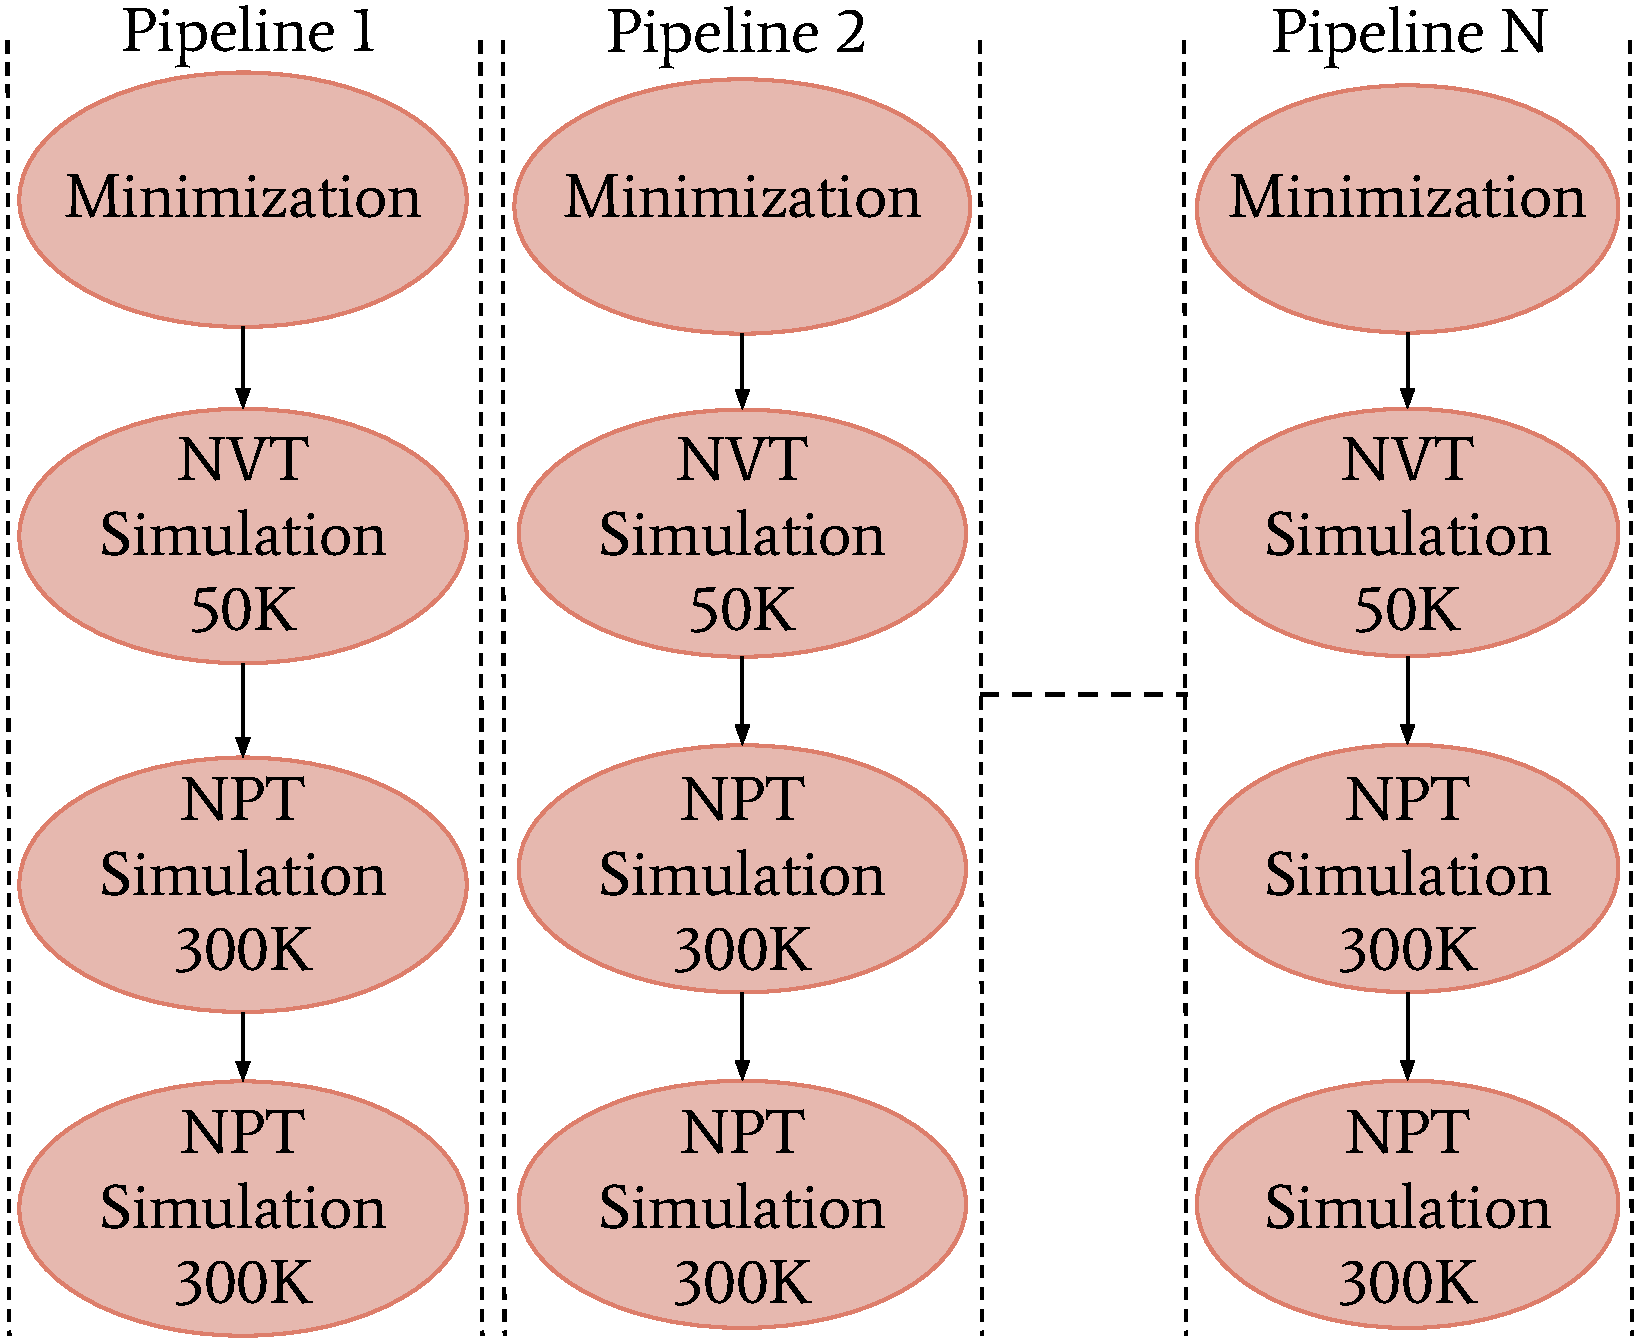
\includegraphics[width=0.5\textwidth]{FIGURES/HT-BAC_NAMD_pipelines_control_flow_only.pdf}
%   \caption{\bf NAMD Stages of HTBAC ESMACS protocol.}
%   \label{figure:ESMACS-pipelines}
% \end{figure}


We define the client resource in Fig~\ref{figure:ht-bac_rp} as the workload
system---HTBAC which describes a series of replicas with ordered functions as
a pipelines with stages and tasks. EnTK interprets these pipelines as a
functional set of tasks and generates the pilot description that contains the
resource configuration of how to run the HTBAC workload. For the ESMACS
protocol running on Blue Waters we define the runtime system, queue, and the
pilot size. Once RADICAL-Pilot receives this new workload it generates a
pilot that submits placeholders to the queue. Once the pilot is activated,
the RP-Agent submits the tasks in the form of compute units to the
placeholders to begin execution.


\begin{figure}
\centering
  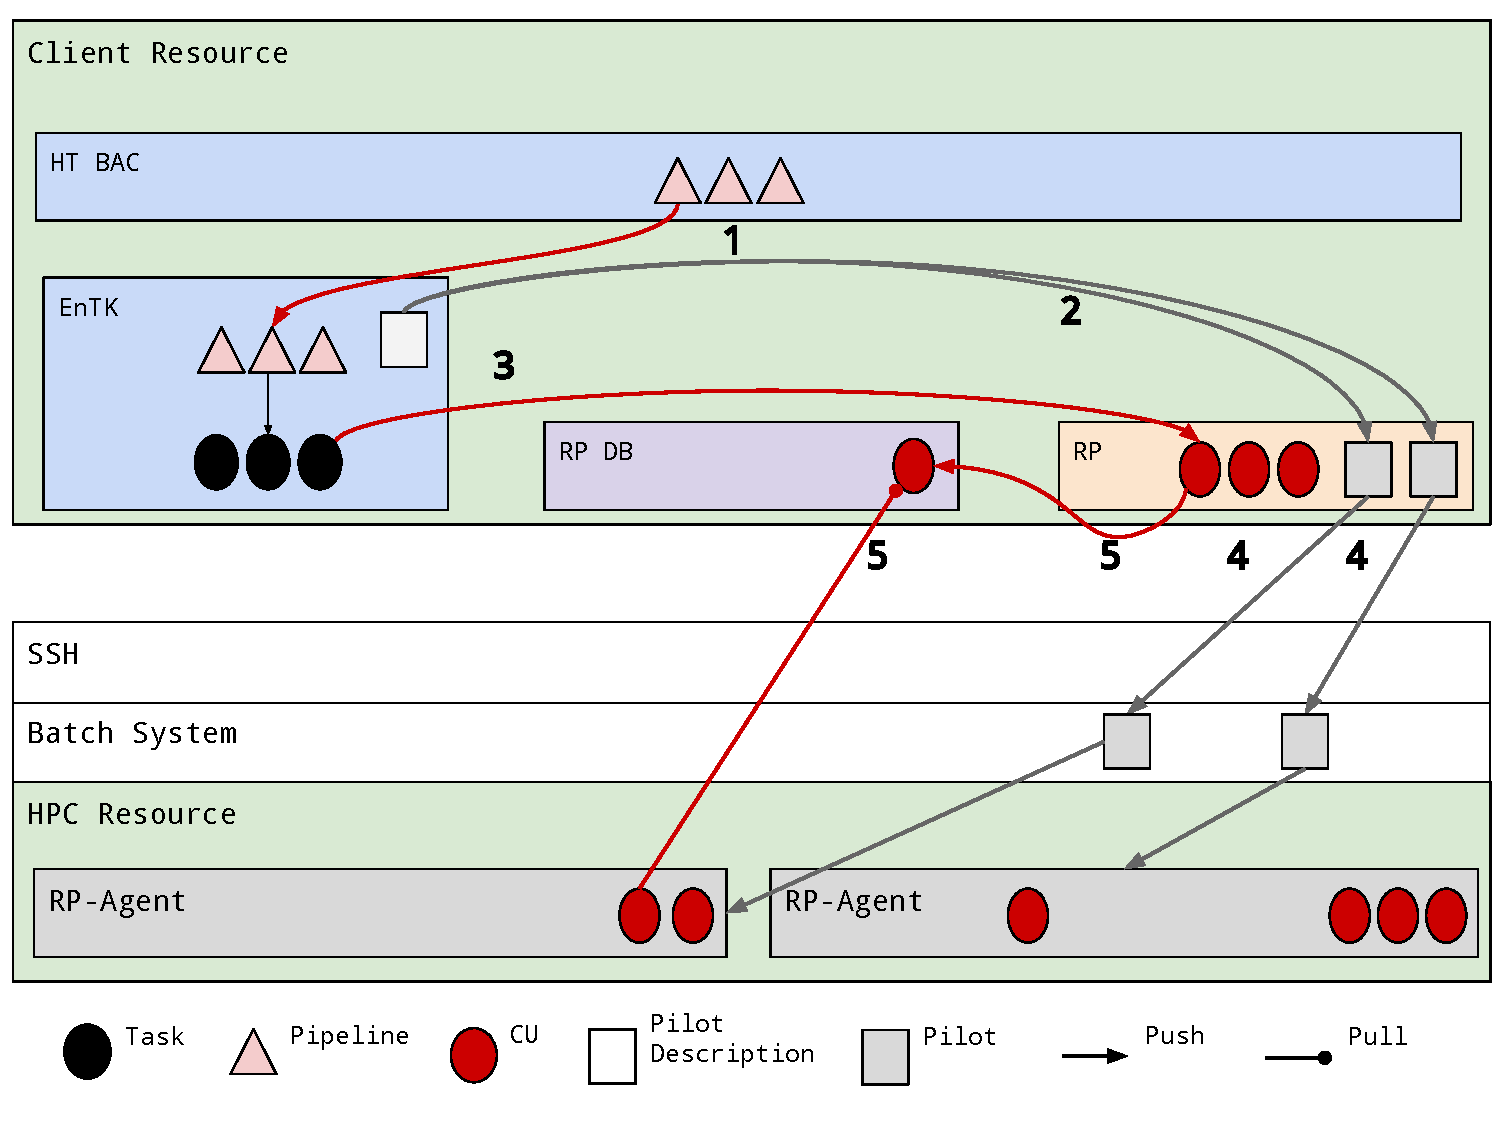
\includegraphics[width=0.5\textwidth]{FIGURES/ht-bac-rp_integration.pdf}
  \caption{Integration between HTBAC workflow and EnTK\@. Numbers
  indicate the temporal sequence of execution. The database (DB) of
  RADICAL-Pilot (RP) can be deployed on any host reachable from the
  resources. RP pushes compute units (CU) to DB and RP-Agent pulls them for
  execution. \dwwnote{I think CU needs to be defined
  here}\mtnote{Better?}}\label{figure:ht-bac_rp}
\end{figure}


RADICAL-Cybertools provides advanced resource management capabilities and,
thereby delivers the necessary high-throughput capabilities required. HTBAC is
integrated with the EnTK component of RCT. 


% \begin{figure}[ht]
% \centering
%  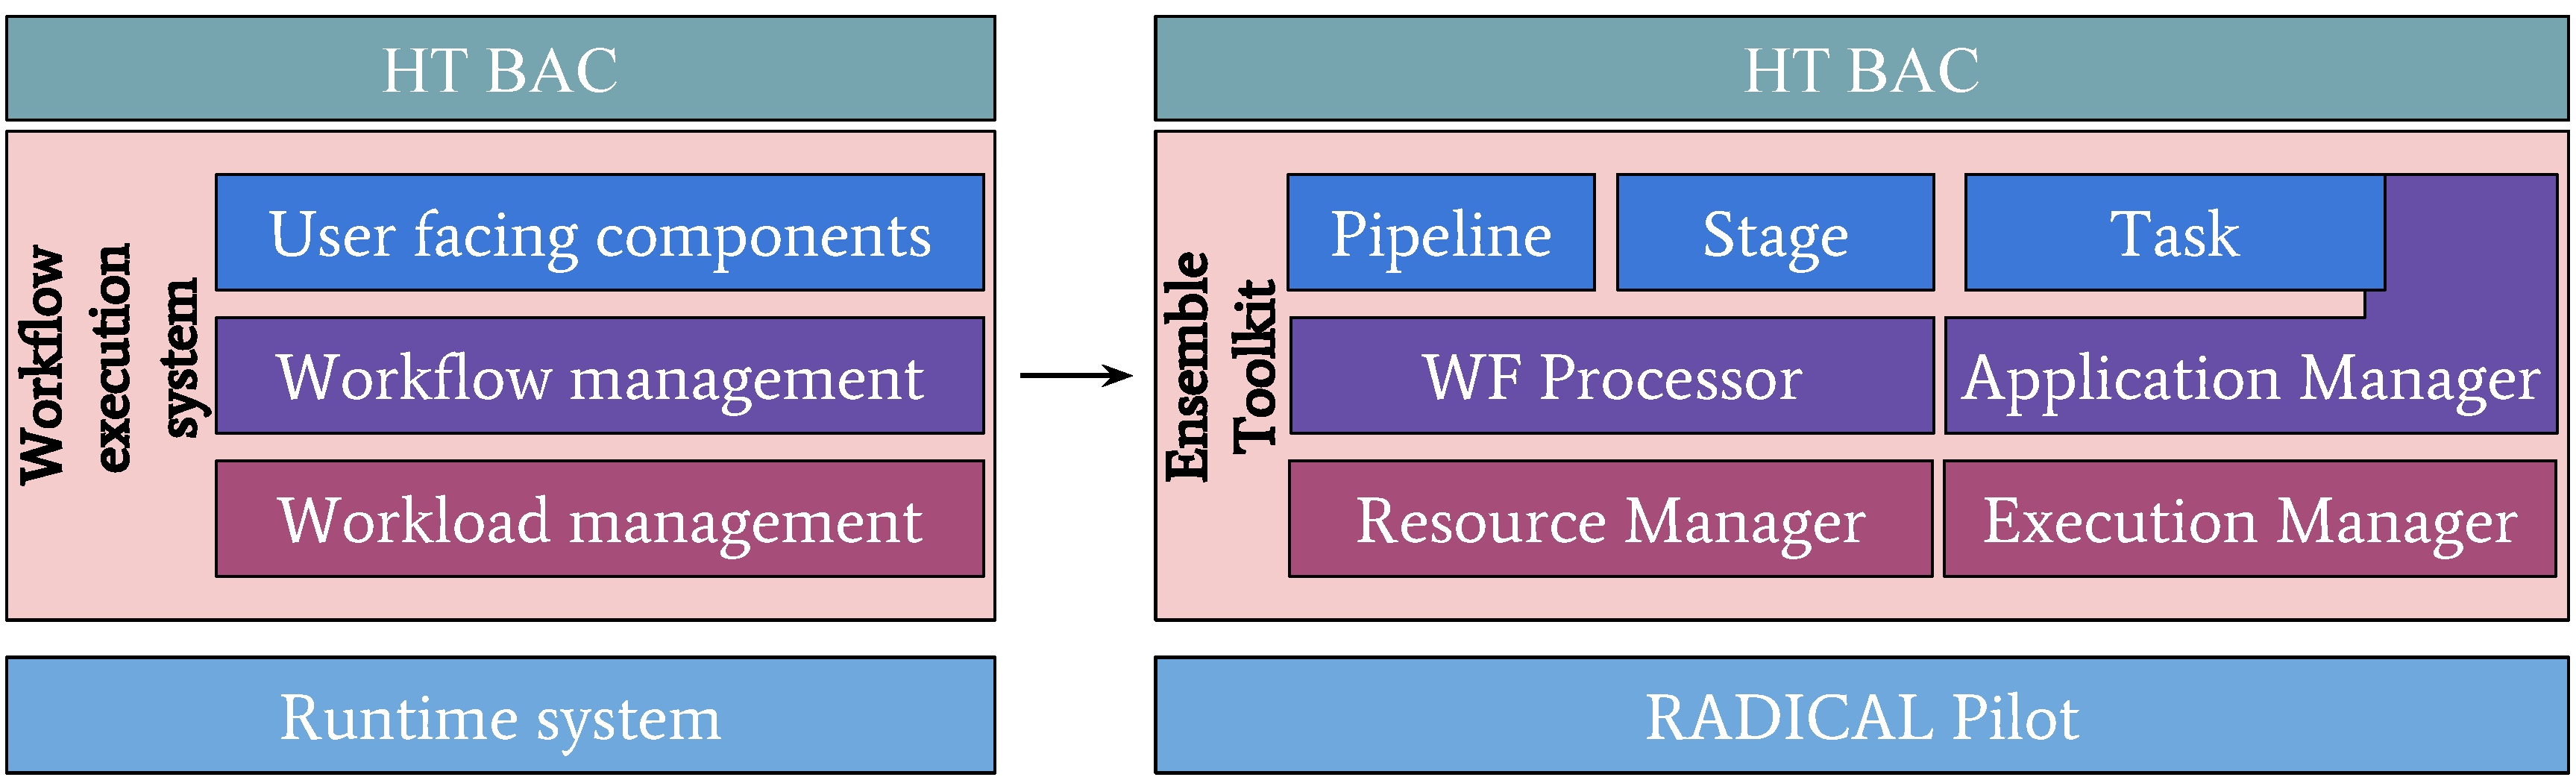
\includegraphics[width=0.5\textwidth]{FIGURES/entk_htbac_integration.pdf}
%   \caption{\bf Integration between HT-BAC workflow system and EnTK that shows resource/application managers.}
%   \label{figure:ht-bac_entk}
% \end{figure}
